\documentclass[tikz]{standalone}

\usetikzlibrary{shapes,arrows,shadows,calc, angles}
\usetikzlibrary{arrows,shapes}
\usetikzlibrary{positioning}
\usetikzlibrary{patterns.meta}
\usetikzlibrary{decorations, decorations.pathreplacing}

\definecolor{fg}{rgb}{0,0,0}
\definecolor{bg}{rgb}{1,1,1}

\tikzstyle{box}=[draw, rounded corners , text width=40mm,
anchor=center,text centered,text=fg, font=\bfseries] % text width=33mm,

\tikzstyle{myarrow}=[->, >=stealth, very thick, rounded corners=2mm]
\tikzstyle{mythinarrow}=[myarrow, line width=0.25mm]

\tikzstyle{conv}=[box, fill=red!60]
\tikzstyle{norm}=[box, fill=yellow!60]
\tikzstyle{concatenation}=[box, fill=cyan!60]

\begin{document}

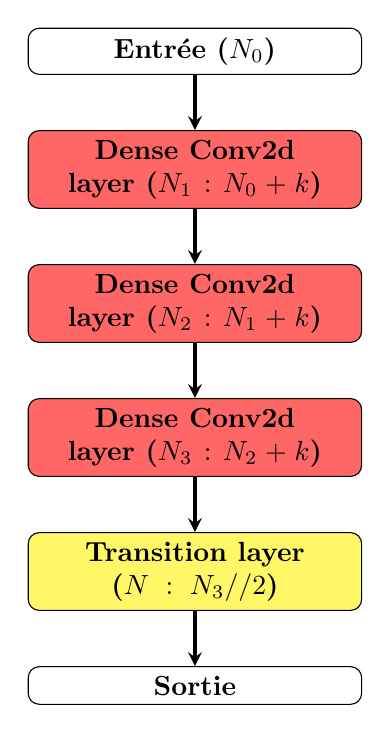
\begin{tikzpicture}[node distance=7mm]

    \node[box] (X) {Entrée ($N_0$)};
    
    \node[conv, below=of X] (conv1) {Dense Conv2d layer ($N_1:N_0+k$)} ;
    \draw[myarrow] (X) -- (conv1) ;
    
    \node[conv, below=of conv1] (conv2) {Dense Conv2d layer ($N_2: N_1+k$)} ;
    \draw[myarrow] (conv1) -- (conv2) ;

    \node[conv, below=of conv2] (conv3) {Dense Conv2d layer ($N_3: N_2+k$)} ;
    \draw[myarrow] (conv2) -- (conv3) ;
    
    \node[norm, below=of conv3] (transition) {Transition layer ($N: N_3 // 2$)} ;
    \draw[myarrow] (conv3) -- (transition) ;
    
    % \draw[myarrow] (conv3) -- (add) ;
    % \draw[myarrow] (X) -- ++ (0, -7mm) -| ++ (-25mm, -15mm) |- (add) ;
    
    \node[box, below=of transition] (Y) {Sortie} ;
    \draw[myarrow] (transition) -- (Y) ;
\end{tikzpicture}

\end{document}